
\subsubsection{\stid{2.08} HPCToolkit} 
\paragraph{Overview} 

The HPCToolkit project is working to develop performance measurement and analysis tools to help ECP software developers understand where and why their programs do not fully exploit hardware resources within and across nodes of extreme-scale parallel systems. Key deliverables of the project are a suite of software tools that developers need to measure and analyze the performance of parallel applications as they execute on existing ECP testbeds and new technologies needed to measure and analyze performance on forthcoming Exascale systems.

To provide a foundation for performance measurement and analysis, the project team is working with community stakeholders, including standards committees, vendors, and open source developers to improve hardware and software support for measurement and attribution of application performance on extreme-scale parallel systems. The project team has been engaging vendors to improve
 hardware support for performance measurement in next generation systems and working with other software teams to design and integrate new capabilities into operating systems, runtime systems, communication libraries, and application frameworks that will enhance the ability of software tools to accurately measure and attribute code performance on extreme-scale parallel systems.  Using emerging hardware and software interfaces for monitoring code performance, the project team is working to extend capabilities to measure computation, data movement, communication, and I/O as a program executes to pinpoint scalability bottlenecks, evaluate resource consumption, and quantify inefficiencies. 




% HPCToolkit as well as the technologies that the project is contributing to the hardware and software ecosystem is needed for ECP because no existing tools are able to measure and precisely attribute the performance of software executing on scalable parallel systems with heterogeneous node-level compute technologies. The project is working to develop tools that attribute performance of code at all levels of the software stack including the application, runtime systems, libraries, and operating systems on  traditional CPUs as  well as accelerators.

\paragraph{Key  Challenges}

In recent years, the complexity, diversity, and the rate of change of architectures for extreme-scale parallel systems have increased dramatically. For higher efficiency, heterogeneous designs that couple multicore processors with accelerators and employ more complex memory hierarchies have been increasing in importance. In addition,  the DOE is purposefully pursuing multiple independent architectural designs for next generation parallel systems as part of risk mitigation. For performance tools, the need to support multiple diverse architectural paths significantly increases tool complexity. 
% For instance, performance measurement and analysis methodologies for accelerators such as graphics processor units that play a central role in the emerging CORAL systems are completely different than methodologies used for measuring the performance on alternative designs in ECP testbeds based on manycore processors.
At the same time, the complexity of applications is increasing dramatically as developers struggle to expose billion-way parallelism, map computation onto heterogeneous computing elements, and cope with the growing complexity of memory hierarchies. While application developers can employ abstractions to hide some of the complexity of emerging parallel systems, performance tools must be intimately familiar with all of the idiosyncratic features added to these systems to improve performance or efficiency, develop measurement and analysis techniques that assess how well these features are being exploited, and then relate these measurements back to software to create actionable feedback that will guide developers to improve the performance, efficiency, and scalability of their applications.

\paragraph{Solution Strategy}

Development of HPCToolkit as part of ECP is focused on preparing it for production use at Exascale by enhancing it in several ways. First, the team is adding new capabilities to measure and analyze interactions between software and key hardware subsystems in extreme-scale platforms, including more complex memory hierarchies and accelerators. Second, the team is working to improve performance attribution given optimized code for complex node-level programming models used by ECP developers, including OpenMP and template-based programming models such as LLNL's RAJA and Sandia's KOKKOS. To support this effort, the project team is enhancing the Dyninst binary analysis toolkit, which is also used by other ECP tools. Third, the team is improving the scalability of HPCToolkit so that it can be used to measure and analyze extreme-scale executions. Fourth, the project team is working to improve the robustness of the tools across the range of architectures used as ECP platforms. Fifth, the team will enhance HPCToolkit's user interfaces to help analyze performance bottlenecks on extreme-scale platforms.  Finally, the project team will work other ECP teams to ensure that they benefit from HPCToolkit's capabilities to measure, analyze, attribute, and diagnose performance issues on ECP testbeds and forthcoming Exascale systems.  

\paragraph{Recent Progress}

Over the last year, the HPCToolkit project has significantly enhanced the ability to measure and analyze application performance. 

\begin{itemize}
\item
The project team added a new measurement substrate to HPCToolkit to measure performance using the Linux perf\_events interface. Using perf\_events enables HPCToolkit to measure operating system activity and thread blocking in addition to application execution. Figure~\ref{fig:hpctoolkit-kernel} displays a screenshot of HPCToolkit's code-centric user interface that shows how HPCToolkit reports information about kernel activity on behalf of an application as part of an application's performance. 
%The screenshot shows that the performance of data movement occurring as part of interprocess communication in a parallel code is a function of how fast a single hardware thread can perform a copy loop within the operating system kernel.
 \item
To accurately attribute code performance to elements of complex, parallel software frameworks that have been transformed  by optimizing compilers, HPCToolkit employs an approach that combines information recorded by compilers about line maps and the provenance of inlined code with direct analysis of machine code to recover information about a program's control flow. Over the past year, the project team has developed improved techniques for recovering control flow graphs from machine code 
 and employed them to relate application performance to inlined functions, templates, and  loops in highly optimized code on both host processors and attached accelerators. Figure~\ref{fig:hpctoolkit-perfsuite} shows the precise attribution of performance measurements to C++ templates employed as part of LLNL's RAJA portability layer.
\item
The project team has developed novel capabilities for measurement, analysis, and attribution of applications that employ graphics processing units (GPUs) as accelerators.  This work includes leading the design of the OMPT tool application programming interface as part of the emerging OpenMP 5.0 standard, developing a measurement infrastructure as part of {\tt libomptarget}---an open source library for offloading code onto accelerators, enhancing HPCToolkit to ingest measurement data from accelerators, and extending HPCToolkit to analyze binaries for NVIDIA's GPUs to attribute performance of offloaded code. Figure~\ref{fig:hpctoolkit-perfsuite} illustrates how HPCToolkit can attribute the performance of code offloaded onto a GPU to the host context that offloaded the computation.
\end{itemize}

\begin{figure}[t]
\centering
\begin{subfloat}[HPCToolkit kernel activity performance metrics.\label{fig:hpctoolkit-kernel}]%{.48\textwidth}
\centering
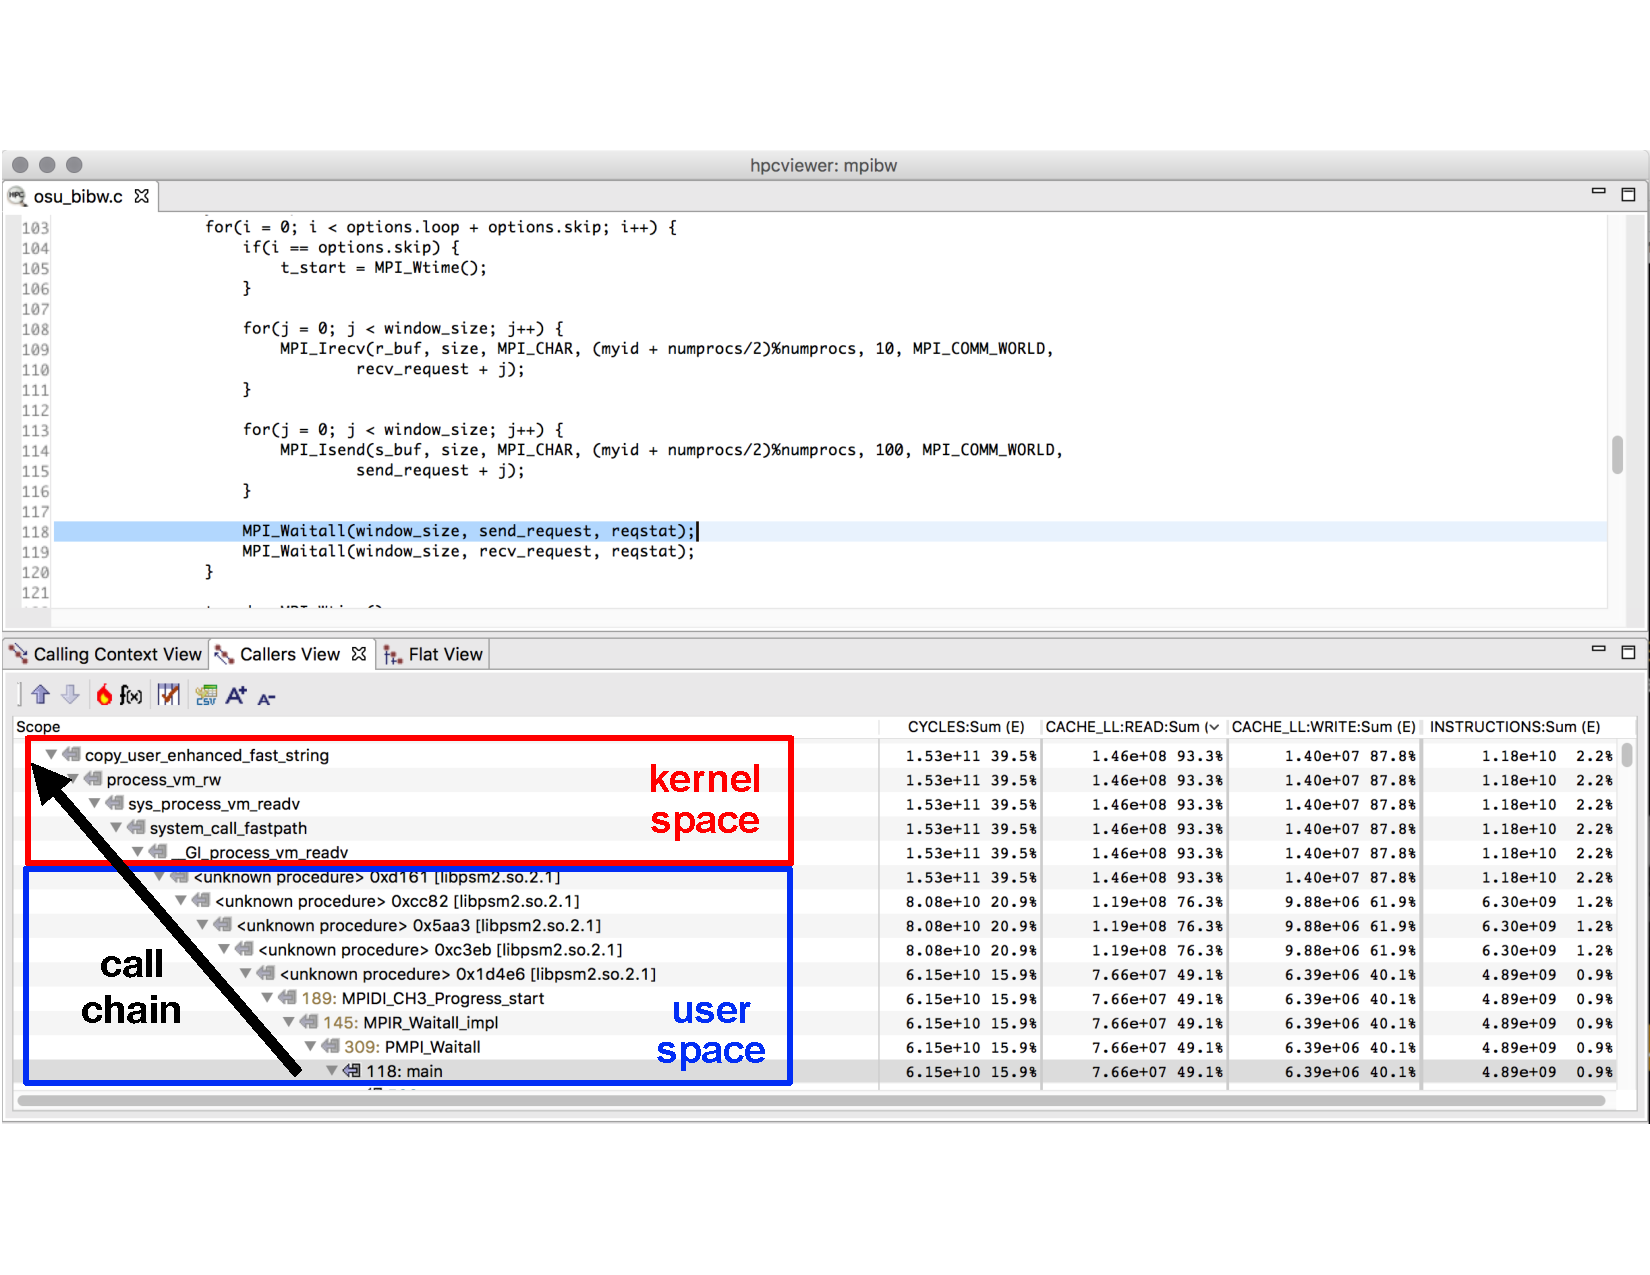
\includegraphics[width=.48\textwidth]{projects/2.3.2-Tools/2.3.2.08-HPCToolkit/hpctoolkit-kernel}
%\caption{The December 2017 release of HPCToolkit includes support for measuring and attributing performance metrics of kernel activity on behalf of an application.}
%\label{fig:hpctoolkit-kernel}
\end{subfloat}
\hfill
\begin{subfloat}[HPCToolkit GPU offloaded performance.
\label{fig:hpctoolkit-perfsuite}]%{.48\textwidth}
\centering
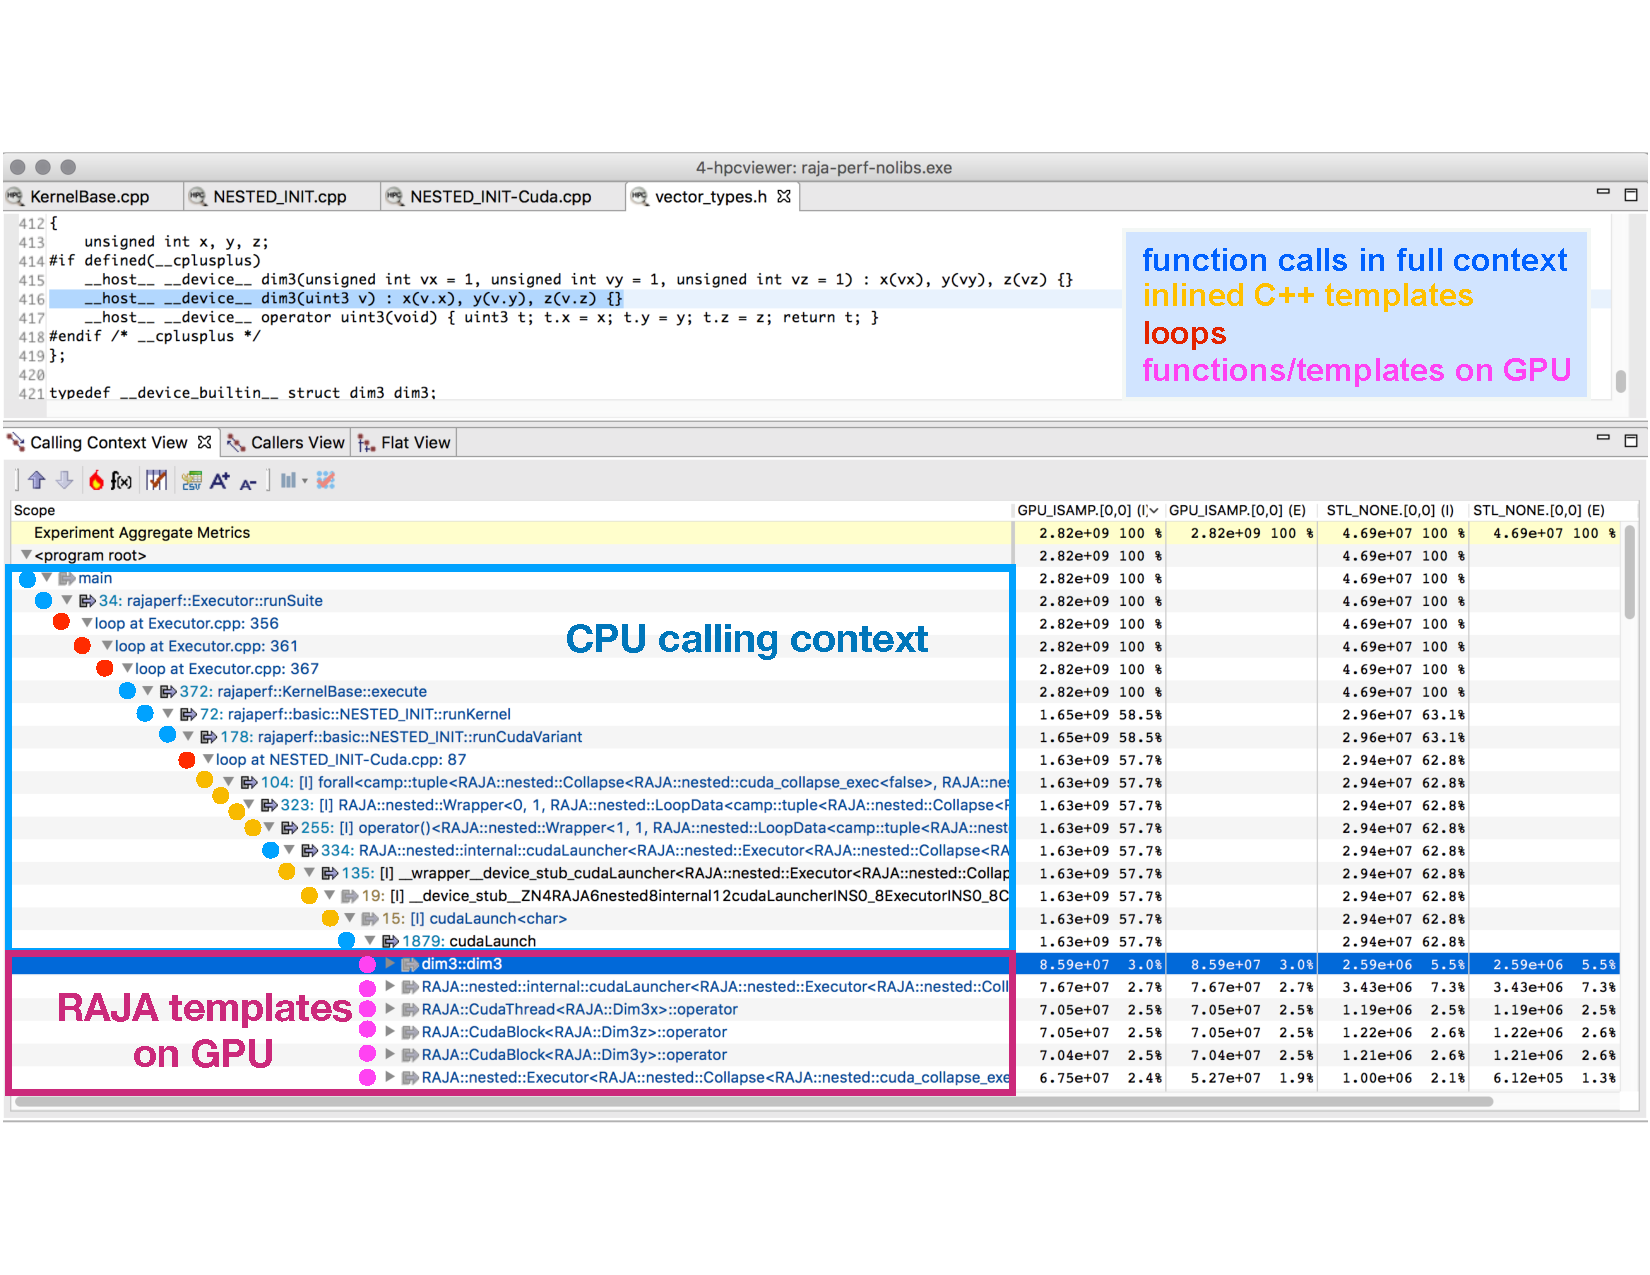
\includegraphics[width=.48\textwidth]{projects/2.3.2-Tools/2.3.2.08-HPCToolkit/hpctoolkit-perfsuite}
%\caption{HPCToolkit now measures and attributes the performance of computation offloaded to GPUs using LLNL's RAJA template-based programming model.}
%\label{fig:hpctoolkit-perfsuite}
\end{subfloat}
\caption{The December 2017 HPCToolkit release supports measuring and attributing performance metrics of kernel activity on behalf of an application.  HPCToolkit now measures and attributes the performance of computation offloaded to GPUs using LLNL's RAJA template-based programming model.}
\end{figure}
\vspace{-1ex}

\paragraph{Next Steps}

The next steps in the project are to:
\begin{itemize}
\setlength\itemsep{0em}
\item Work with the OpenMP standards committee to finalize tool interfaces as part of the emerging OpenMP standard.
\item Complete and deploy implementation of  HPCToolkit's support for measurement and analysis of code offloaded onto NVIDIA GPUs. 
%Work to integrate GPU measurement support back into the open-source {\tt libomptarget} library.
\item Integrate new support for task-based parallelism developed as part of the project's Dyninst binary analysis infrastructure into HPCToolkit's binary analyzer to accelerate analysis of large executables.
\item Complete work on data-centric performance analysis capabilities that  measure and attribute data movement costs to program variables.
\item Complete and deploy a framework for regression testing of HPCToolkit.
\item Work with DOE and Intel on performance measurement technologies for the A21 Exascale platform.
\end{itemize}
